\chapter{Formal Phrase Replacement}

\label{Chapter06}

\section{Problem}

To change an entirely formal sentence to an entirely informal one could require, as seen in Section \ref{gyafc} about the GYAFC and Chapter \ref{Chapter03} about my work with that same dataset, complete transformation of a sentence, from syntactic structure to almost every individual word. Yet this comes with a risk of losing the meaning or fluency of the original sentence, and the level of informality could end up too high for the use cases relevant to this project.

In Chapter \ref{Chapter04} I found that when focusing on narrowing formality translation to the phrasal level, one of the largest categories of edits involved replacing certain formal words or phrases with corresponding informal ones (see Table \ref{acro-edits-table}). This was the second category that I chose as a task for this project: formal phrase replacement. That is, given a sentence, what phrase can be replaced with another to make the sentence more informal?

For this task I developed a two-part system, the first part of which locates the span containing a formal phrase in a sentence, and the second of which translates that segment to a less formal equivalent. Even moreso than the discourse marker insertion problem, this problem would ideally necessitate a large dataset manually validated by humans. Given that this was not possible within the scope of this work, the bulk of the work for this task was to automatically assemble a dataset as close to these ideals as possible, and focus on whether or not a model could be taught to generalize from these data.

% write something about the overall takeaway here

\section{Data}

The desired data format for this task is a sentence, a span marking the location of a formal phrase therein, and a phrase which could exactly replace that span and is also less formal than the original. This matches the format of the Acrolinx Blog Post Dataset. As there is not an existing dataset that fits this description --- the edits in the Acrolinx Blog Post Dataset which are in this category number only 441 --- one had to be compiled.

As an overview, the dataset was formed by taking a list of formal words and their informal replacements, finding each occurrence of each phrase in a collection of sentences, marking the larger phrases they were found in, and then replacing them within each phrase. I will detail the specifics of that process in this section.

\subsection{Initial Seed Words}

First, a set of seed formal words and phrases with informal replacements had to be gathered. Acrolinx, as described in Section \ref{acrolinx}, has existing lexicons with formal words and phrases, some of which already have suggested replacements. I gathered all of these terms, and those which had replacements were the original seed set. There were 258 terms and replacements in the original seed list.

\subsection{Phrase List Expansion}

The initial seed word list needed to be expanded to ensure a better variety of words and phrases, but not so much that it could not be manually validated in an efficient length of time. A list of potential expansion words started from the words in the Acrolinx lexicons that did not have informal replacements. Next, the Microsoft corpus was run through Acrolinx and the words that it marked as formal, according to the Lexical Formality score described in Section \ref{lf}, were also added to the potential expansion words. The subtask was the to extend the relationship between the paired words and phrases in the seed list to the potential additions.

To do this, I used word embeddings: specifically, a pretrained model from the developers of word2vec, which had vectors of 300 dimensions and was trained on the Google News corpus (\cite{mikolov2013word2vec}). Using simple vector math, one can create analogies of words. For example, consider the analogy: ``obtain'' is to ``get'', as ``purchase'' is to what word? By subtracting the vector for ``obtain'' from ``get'' and then adding the vector for ``purchase'', we find a point in the vector space. Looking at the words which are located closest to that point, we --- theoretically, as it does depend on the word embedding --- find the word ``buy''.

Thus, using this method for all the potential additions, the top 10 possible informal replacements for each term were collected. This method did mean that only single words were possible to add, and not whole phrases, as they do not have embedding vectors alone. As such, the list contains mostly single words and single word replacements, significantly more than it does phrases. From this, I looked over the list and kept only those words which were appropriate replacements, that kept the meaning intact while reducing formality. The edits from the Acrolinx blog post data were also added to this list.

Importantly, this meant that the final list sometimes offered more than one potential replacement word for any given formal word. Sometimes this was for grammatical reasons --- as ``commenced'' might require ``begun'' or ``began'', depending on the verb form --- and sometimes it was because there was more than one informal option.

One more manual verification step had to be completed before the list of formal words/phrases and informal replacements could be considered complete. I checked that each replacement could happen independent of context, or that in most contexts, at least one of the potential informal words or phrases could be inserted in the formal word or phrase's place.

The final list consisted of 827 formal phrases with informal replacements.

\subsection{Collected Sentences}

Similar to the discourse marker insertion approach, I took data from the British National Corpus and the Open American National Corpus (\cite{bnc}, \cite{ide2001oanc}). As this task did not require information at the paragraph level (which sentences come consecutively), I also added the sentences from the Brown corpus as provided through NLTK (\cite{bird2009nltk}, \cite{francis1979brown}). After removing items that were not actual sentences through preprocessing, the total number of sentences was approximately 3.8 million.

\subsection{Dataset Compilation}

Given the list of formal words/phrases and their informal replacements, it becomes simple with rule-based methods to simply identify those words and put any of the possible replacements in their place. However, this may not always be accurate, if there are multiple options for replacements not all of them may be appropriate for every context, and it would be restricted to only the words on the original list. With this task, the hope was to extrapolate beyond that, and to identify and translate other phrases.

Giving an informal replacement requires more than just a formal word, then: some context is needed. The collected list had some phrases, but mostly single words due to the use of word embeddings to expand it. On the other hand, giving the whole sentence only brings one back to the problem at the heart of this project: the risk of corrupting the meaning or grammar of the sentence. With that said, I chose to extract the syntactic phrases which the words were located in.

A package called spaCy was used to compute the dependency parse tree for each sentence (\cite{honnibal2017spacy}). If any formal words from the word list were found in the sentence, the nearest phrase in its dependency structure was marked as formal. More specifically: if it is in a noun phrase, then that phrase was marked. Otherwise, to ensure that a continuous segment was found, the nearest subtree was marked, looking first to the right and then to the left.

Marked locations are recorded in labels that match the sentence length, wherein each label is a binary indicator for whether or not its corresponding token belongs to a formal phrase.

\begin{table}[h]
\centering
 \begin{tabular}{|| p{8cm} | p{4cm} ||}
 \hline
 Sentence & Replacement \\ [0.3ex] 
 \hline\hline
 Her mother had taken great care \textbf{to provide a lot of love} and attention to Mary, often at the neglect of the baby. & to give a lot of love \\
 \hline
 Lose weight more quickly than ever before, because a larger proportion of \textbf{the calories you consume will remain} undigested. & the calories you consume will stay \\
 \hline
 This machine, \textbf{operating at speeds up to 350,000 revolutions per minute}, is believed \textbf{to provide one of the fastest} mechanical operations in industry today. & working at speeds up to 350,000 revolutions per minute \newline to give one of the fastest \\
 \hline
\end{tabular}
\caption{A few examples of sentences from the collected data for the Formal Phrase Replacement task. Marked formal phrases are in bold, with their replacements in the second column.}
\label{lexical-data-examples}
\end{table}

In the end, the dataset comprised 525,114 sentences from the three original corpora. With duplicates removed, the number of phrases with informal translations was 306,715. Some examples of sentences with marked formal phrases and their replacements are given in Table \ref{lexical-data-examples}.

\subsection{Vectorization}

For this task word2vec word embeddings were trained using gensim (\cite{mikolov2013word2vec}, \cite{rehurek2010gensim}). Vector dimension size was set to 100 with a context window of 5. Minimum number of appearances in the data in order to be counted in the vocabulary was also set to 5. The model was trained for 10 epochs over the entire set of sentences. In the end, the vocabulary size was a little under 150,000.

\subsection{Small Dataset}

A problem with the dataset was that phrases which included some words occurred far more often than others. Phrases centered around the word ``abaft'', for example, occurred less than five times, whereas ``thus'' was in thousands of sentences. To reduce the impact of this problem, and to see if overfitting to the phrase list could be preemptively avoided, a much smaller version of the dataset was compiled.

This time, when going through the sentences, if every formal word whose phrases were marked in the sentence occurred over 10 times in the dataset already, then it was not included. After this process the smaller dataset was complete at only 7146 sentences total.

\section{Methods}

As discussed, this task was split up into two models: one that would identify formal phrases in sentences, and a second that would take those formal phrases alone and translate them into informal equivalents.

\subsection{Phrase Identification}

\begin{figure}
    \centering
    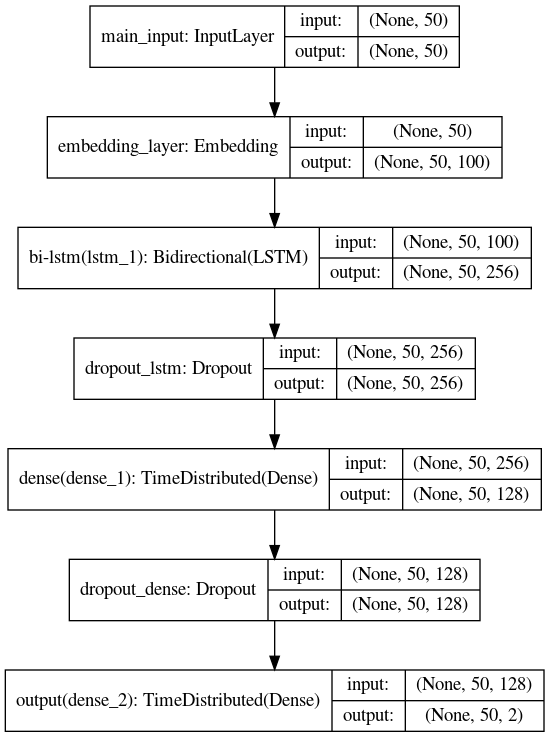
\includegraphics[width = 10cm]{Figures/graph-lexical.png}
    \caption{Visualization of the architecture for the models used to train for the formal phrase replacement task. Note that ``None'' represents the batch size.}
    \label{fig:lexical-architecture}
\end{figure}

A neural network was constructed for the task of finding the formal phrases within sentences. The maximum sentence length was set to 50; longer sentences were cut off and shorter sentences were zero-padded to that length. The architecture included a bidirectional LSTM with 128 units (each direction) and dropout (with a keep probability of 0.75), followed by a dense layer over the sequence with 128 units and dropout with rectified linear units as the activation function, and lastly a softmax output layer. A visualization of this architecture can be seen in Figure \ref{fig:lexical-architecture}.

The model was trained for one epoch over the entire dataset, which took about 45 minutes.

\subsubsection{Reduced Model}

Another model was trained on the small dataset, with some additional changes to the architecture. The number of units in the LSTM and dense layers was halved, so that it was 64. This was done, similar to the reasoning behind creating the small dataset in the first place, to reduce the capacity of the model to make it less likely to simply memorize the smaller amount of data. Otherwise, the architecture was the same. The model was trained for three epochs, which took altogether approximately three minutes.

\subsection{Phrase Replacement}

As the phrase replacement problem can be viewed a neural machine translation problem, only on the phrasal level instead of the typical sentential focus, I used OpenNMT for this part of the task (\cite{2017opennmt}). Default parameters were kept aside from the addition of copy attention, as before to allow the model to copy the parts of the phrase that should stay constant.

Training the model took about three hours, through 100,000 iterations. Notably, this was not even the full length of the dataset, but it was suspected that at that point more similar phrases would not have added any information to the model; furthermore, completing an epoch and doing a second run over the dataset might have enabled the model into memorizing the training set.

\subsubsection{Reduced Model}

Another model was trained that was identical to the ``main'' model, with the same OpenNMT parameters and training dataset, except instead of training for 100,000 iterations, it was only trained for 5000. Just like with the phrase identification model on the smaller dataset, this was meant to see if giving less information would make it less likely that the model only learns to replace the original word list instead of generalizing to other formal to informal translations.

\section{Results}

This section provides results for the main and the reduced models in order to compare them and evaluate how both models for both subtasks performed.

There were essentially two questions that needed to be asked in order to evaluate these models. First, did the models learn the initial list of formal phrases? This would be the baseline, what a rule-based formalism could accomplish: can the models identify and replace those words which were marked and translated in the dataset? To answer this question, results on the test datase in particular can be examined to see if a high degree of accuracy was achieved.

The second question is arguably more important, and it is: were the models able to move beyond the wordlist and generalize to other formal phrases and their informal translations? For this problem, the Microsoft data is used to see what else the models were able to learn.

% what did i find overall?

\subsection{Phrase Identification}

The first of our questions is addressed by evaluating results on the test and training sets.

\begin{table}[h]
\centering
 \begin{tabular}{|| l | r | r ||}
 \hline
 Term & train & test \\ [0.3ex] 
 \hline\hline
 Size & $472602$ & $52512$ \\
 \hline
 Accuracy (sentence level) & $69.2$ & $68.9$ \\
 \hline
 Accuracy (token level) & $97.6$ & $97.5$ \\
 \hline
 Precision (token level) & $86.8$ & $86.3$ \\
 \hline
 Recall (token level) & $88.6$ & $88.4$ \\
 \hline
 Avg errors per sentence & $1.22$ & $1.25$ \\
 \hline
\end{tabular}
\caption{Results for the phrase identification model which was trained on the full dataset. Accuracy at the sentence level is achieved if the model makes no errors over the full sentence.}
\label{phrase-ident-main-results}
\end{table}

Results are given in Table \ref{phrase-ident-main-results}. The default accuracy, at the token level, can be misleading, since the formal phrase(s) mark for the most part only a small portion of the sentence's length. Precision and recall help give a clearer perspective of the model's performance, but two other metrics were calculated in order to provide more information. One was accuracy at the sentence level, in which a sentence is considered correctly predicted if the label of every word has been predicted correctly. The other is the average number of incorrect labels per sentence.

These results show little overfitting (results on the train and test sets show only very small differences). While the numbers look impressive at first glance, this also suggests the opposite of what was desired: that the model did not generalize to phrases beyond the initial list used to assemble the dataset. If it had, the accuracy values, particularly for the test set, would be lower, as phrases which were not originally marked in the set would have been found and marked by the model.

\begin{table}[h]
\centering
 \begin{tabular}{|| l | r | r ||}
 \hline
 Term & train & test \\ [0.3ex] 
 \hline\hline
 Size & $6431$ & $715$ \\
 \hline
 Accuracy (sentence level) & $25.1$ & $21.7$ \\
 \hline
 Accuracy (token level) & $94.3$ & $92.7$ \\
 \hline
 Precision (token level) & $73.7$ & $62.4$ \\
 \hline
 Recall (token level) & $60.1$ & $55.6$ \\
 \hline
 Avg errors per sentence & $2.87$ & $3.65$ \\
 \hline
\end{tabular}
\caption{Results for the less complex phrase identification model which was trained on the reduced dataset. Accuracy at the sentence level is achieved if the model makes no errors over the full sentence.}
\label{lexical-ident-reduced-results}
\end{table}

For the reduced model, outcomes can be seen in Table \ref{lexical-ident-reduced-results}. As expected, results are worse across the board. Note in particular the large difference in sentence-level accuracy between this and the main model, as opposed to the small difference in token-level accuracy; the presence of the additional metrics makes it clear that this model did not learn as much as the previous. To clarify what exactly was learned and to answer the second of our questions, supplementary tests were run on the Microsoft corpus.

\subsubsection{Tests on Generalization}

\begin{table}[h]
\centering
 \begin{tabular}{|| l | r | r ||}
 \hline
  & Main & Reduced \\ [0.3ex] 
 \hline\hline
 Total Phrases Identified & $7093$ & $10197$ \\
 \hline
 Number of Generalized Phrases & $847$ & $4308$ \\
 \hline
 Percent Generalized Phrases & $11.9\%$ & $42.2\%$ \\
 \hline
\end{tabular}
\caption{Sentences from the Microsoft dataset were used as test data for both the main and reduced models for phrase identification, in understanding what the models were able to learn.}
\label{mic-phrase-ident}
\end{table}

10,000 sentences were randomly sampled from the Microsoft corpus for these tests, as to provide data for testing that is from a different source altogether from the training data. The purpose was to see, for both models, whether or not they were identifying phrases that went \textit{beyond} the initial word list used to create their training datasets. In the table, these are referred to as ``Generalized Phrases''. Results show that despite the constraints on the training data, both models were able to identify phrases which did not merely center around the wordlist. And as expected, the less powerful model trained on the reduced dataset picked up more than the full model.

\subsection{Phrase Replacement}

NMT approaches still present a difficulty with automatic evaluation; the case against BLEU for formality translation has already been presented in this report. This particular use, however, with its restricted scope, meant an easy method of evaluation presented itself.

\begin{table}[h]
\centering
 \begin{tabular}{|| l | r | r ||}
 \hline
  & 100k-iter & 5k-iter \\ [0.3ex] 
 \hline\hline
 Accuracy & $93.1$ & $91.5$ \\
 \hline
\end{tabular}
\caption{Binary accuracy results for the OpenNMT phrase replacement models.}
\label{phrase-repl-results}
\end{table}

To answer the first question --- has this model at least learned the word list? --- the output of the models on the test set was put to a simple test: was the word from the initial wordlist replaced within the original phrase, and all other words kept the same? The output of the 30,000 test sentence was used for this evaluation, and the results are given in Table \ref{phrase-repl-results}. The model trained on 5000 iterations was only slightly worse than the one trained on 100,000, showing that not much data at all was needed for the OpenNMT models to learn the initial word list.

\begin{table}[h]
\centering
 \begin{tabular}{|| l | r | r ||}
 \hline
  & 100k-iter & 5k-iter \\ [0.3ex] 
 \hline\hline
 Percent Changed & $43.4\%$ & $49.6\%$ \\
 \hline
\end{tabular}
\caption{How many phrases the translation models changed from the Microsoft formal phrases, as marked by the phrase identification systems.}
\label{phrase-repl-mic-test}
\end{table}

Next, the second question must be answered --- has this model gone beyond the word list? To address this, I collected the phrases marked as formal by both main and reduced phrase identification models on the Microsoft sample sentences. Skipping the phrases which only included one word, the final set contained 2010 phrases. The next check was to see if the input phrases were at all changed, or if the models simply copied them into the output. Although this does not evaluate whether or not any changes were sensible or not, the results of this basic test are included in Table \ref{phrase-repl-mic-test}.

An important caveat comes with these tests: it operates under an assumption that the phrases found by the phrase identification models in the previous part are correctly identified as formal, which may not be the case (in which case there would be nothing to translate, and the copying of the input to output would be a correct action). Still, the results do provide information. First, that the 5k-iter model changed more than the longer-trained model fits in line with the expectation that it had a reduced capacity for learning to only change the words from the initial list. Second, despite that observation, the difference between the two models is far less than that of the main and reduced phrase identification models. Similar to the accuracy results presented in Table \ref{phrase-repl-results}, this supports the finding that reducing the number of iterations to only 5000 did not make a huge difference. But without looking into the results qualitatively, as will be done in the next section, this alone is not enough to say that the models were able to generalize.

\section{Discussion}

In analyzing the results of the efforts for this task, there are two points to address, which conveniently correspond to the two questions focused on in providing results. The first of these concerns the small, but present error rate found when testing for the initial word list; the source of these mistakes should be examined. The second topic is regarding generalization, and entails honing in on what exactly the models have learned. Both of these topics are addressed for both subtasks here.

\subsection{Errors in Phrase Identification}

\begin{table}[h]
\centering
 \begin{tabular}{|| p{4cm} | p{4cm} | p{4cm} ||}
 \hline
 True Label & Main Model Output & Reduced Model Output \\ [0.3ex] 
 \hline\hline
 How is \textbf{the child's performance on the activity assessed}? & 
 How is the child's performance on \textbf{the activity assessed}? & 
 How is the child's performance on \textbf{the activity assessed}? \\
 \hline
 The footsteps went down, past the kitchen, into the shop; she thought they might vanish altogether but they shortly returned, \textbf{accompanied by a padding, clicking sound}, paws on linoleum. & 
 The footsteps went down, past the kitchen, into the shop; she thought they might vanish altogether but they shortly returned, \textbf{accompanied by a padding}, clicking sound, paws on linoleum. & 
 The footsteps went down, past the kitchen, into the shop; she thought they might vanish altogether but they shortly returned, \textbf{accompanied by a padding}, clicking sound, paws on linoleum. \\
 \hline
 But the Coroner says that for the time being\textbf{, Marc's death will remain a} mystery. & 
 But the Coroner says that for the time being\textbf{, Marc's death will remain a} mystery. & 
 But the Coroner says that for the time being, Marc's death \textbf{will remain a mystery}. \\
 \hline
 Does the ‘abc’ badge \textbf{provide any more comfort for the decision maker?} & 
 Does the ‘abc’ badge \textbf{provide any more comfort for the decision maker?} & 
 Does the ‘abc’ \textbf{badge provide any more comfort for the decision} maker \\
 \hline
\end{tabular}
\caption{Examples of errors made by the phrase identification models, in which they correctly identified the word from the initial list but did not match the phrase boundaries from the true label.}
\label{errors-phrase-ident}
\end{table}

As mentioned previously, the task of finding all words from a given list in a corpus should be a trivial one for a model. With that said, it would be curious that (as shown in Table \ref{phrase-ident-main-results}) accuracy at the sentence level was only 70\% for the main model. However, the task had been extended to find not only the formal words, but the phrases that contained them, so that at the next step, the context required to properly translate the word would be provided. In fact, most of the errors that the main and reduced phrase identification models made turned out to be differing placements of start and end boundaries for those phrases, wherein the main formal word was still included.

With the larger training set, it is unsurprising that the main model would pick up better on the syntactic rules (originally marked by spaCy's dependency parser) that were used to gather the data. The reduced model, while learning the words, does not seem to have achieved this goal to the same degree. Two examples where the reduced model did not match the true label but the main model did and two examples where both models misjudged boundaries are given in Table \ref{errors-phrase-ident}.

\subsection{Errors in Phrase Replacement}

\begin{table}[h]
\centering
 \begin{tabular}{|| p{4cm} | p{4cm} | p{4cm} ||}
 \hline
 source & target & pred \\ [0.3ex] 
 \hline\hline
 to \textbf{exclude} opinion evidence that sought & 
 to \textbf{keep out} opinion evidence that sought & 
 to \textbf{keep} opinion evidence that sought \\
 \hline
 to \textbf{ensure} that where the premises & 
 to \textbf{make sure} that where the premises & 
 to \textbf{make} that where the premises \\
 \hline
 to \textbf{determine} whether a payment made & 
 to \textbf{find out} whether a payment made & 
 to \textbf{find} whether a payment made \\
 \hline
\end{tabular}
\caption{Examples of errors made by the OpenNMT-trained phrase replacement models.}
\label{errors-phrase-repl}
\end{table}

With how stringently both phrase replacement models appeared to have memorized the initial list of formal words, even an accuracy of 90\% seems strange. An inspection of the predicted outputs reveals that most of the errors occurred when a multiple-word replacement for a single-word input was meant to happen. For example, instead of replacing ``ensure'' with ``make sure'', only ``make'' was added. A few examples of this phenomenon can be seen in Table \ref{errors-phrase-repl}.

Both the 100k-iter and 5k-iter models had this problem. It is possible that the inclination which the models learned to replace each word with a single-word replacement (as this was the case for the vast majority of examples) outweighed their memorization of the formal list.

\subsection{Generalization in Phrase Identification}

A problem with the results by the phrase identification models on the Microsoft sentences as shown in Table \ref{mic-phrase-ident} is that the category of ``Generalized Phrases'' would also contain most of the true errors made by the model. Since this category is automatically determined by checking if any words from the initial list appear in the phrase, improperly labeled phrases would also be put in it. This includes phrases which are actually not formal, a type of phrase difficult to discern without manual validation. It also includes cases in which the model ``split'' a phrase by, apparently randomly, marking a word within a formal phrase as informal, and causing it to be recognized as two separate phrases. Here is an example of this:

\begin{quote}
\textbf{The} JSON \textbf{structure that contains information about the conditions} when the start of speech was detected .
\end{quote}

In this case, ``The'' and ``structure that contains information about the conditions'' would be marked as two separate formal phrases. The above example is from the reduced model, which was more guilty of this error than the main model, particularly with unknown tokens such as ``JSON''.

\begin{table}[h]
\centering
 \begin{tabular}{|| p{5cm} | p{5cm} ||} 
 \hline
 Main Model & Reduced Model \\ [0.3ex] 
 \hline\hline
 key attestation & perform operations \\ 
 \hline
 the stored procedure & the incoming queries \\ 
 \hline
 asynchronous & these parameters \\ 
 \hline
 tabulated & evaluate the cost of your \\ 
 \hline
 expiry & if supported for some applications \\ 
 \hline
 recovery & inherited \\ 
 \hline
 log & predictive analytics \\ 
 \hline
 Remove the record & Linux \\ 
 \hline
 classifies the data that & concurrency control \\ 
 \hline
 proxy authentication using machine context & securing your PaaS web and mobile applications \\ 
 \hline
\end{tabular}
\caption{Some examples of phrases marked as formal by both phrase identification models on the Microsoft data.}
\label{phrase-ident-mic-examples}
\end{table}

Besides those errors, though, the formal phrases identified by both models do appear to be genuinely formal. In my observations, the reduced model performed better at still identifying whole phrases to provide some context for the next step. Some errors were certainly made (of this list alone ``log'' and ``Linux'' stick out as not particularly formal). With more work and tuning, the reduced model could better be able to identify formal phrases that it has never seen.

\subsection{Generalization in Phrase Replacement}

\begin{table}[h]
\centering
 \begin{tabular}{|| p{4cm} | p{4cm} | p{4cm} ||}
 \hline
 source & pred 100k-iter & pred 5k-iter \\ [0.3ex] 
 \hline\hline
 is not \textbf{deleted} & 
 is not \textbf{swapped} & 
 is not \textbf{left} \\
 \hline
 \textbf{define} the statement & 
 \textbf{show} the statement & 
 \textbf{describe} the statement \\
 \hline
 the \textbf{repository} & 
 the \textbf{field} & 
 the \textbf{replacement} \\
 \hline
\end{tabular}
\caption{Examples of output on the Microsoft formal phrases by the phrase replacement models.}
\label{general-phrase-repl}
\end{table}

Although the phrases from the Microsoft data were translated by the replacement models, a closer inspection of the output reveals that these translations are, optimistically put, misguided. A sampling of phrases is given in Table \ref{general-phrase-repl}. The patterns laid out here continue in the predicted data. The correct part of speech is maintained, and in terms of meaning, some vague idea seems to be preserved --- but, crucially, the only new words that both models provide are those which it learned to introduce in training.

One important thing to consider is that the default OpenNMT parameters were likely large enough that its capacity was too high for this task and dataset. A multi-layered encoder-decoder system with 500 units in each one, larger than any other model developed in this work, might have been more easily and quickly able to memorize the dataset, or at least only memorize the replacement words. This is something that will have to be more carefully tuned in the future.

\section{Future Work}

The primary task to continue with this research would be to better the dataset.

of course dataset stuff
backtranslation
hyperparameter optimization
if opennmt: mess with more parameters to make less powerful

\section{Takeaway}
